\documentclass[11pt]{article}

\usepackage[margin=1in]{geometry}
\usepackage{amsmath}
\usepackage{booktabs}
\usepackage{float}
\usepackage{graphicx}
\usepackage{hyperref}
\usepackage{natbib}
\usepackage{url}

\title{Gate-State Causal Propagation in a Structured Recurrent Substrate}
\author{Author metadata to be supplied before submission}
\date{May 15, 2026}

\begin{document}

\maketitle

\begin{abstract}
Structured recurrent systems can expose stable or similar readouts while
preserving distinct internal state dynamics. We report Gate-State Causal
Propagation, a replicated mechanism discovered in a five-channel recurrent
substrate with \texttt{fast}, \texttt{slow}, \texttt{control},
\texttt{message}, and \texttt{carrier} state. Under a Track B
native-emergence protocol, three independent replications passed a mechanism
gate: held-out route-disabled and gain-zero divergence remained positive in
3/3 runs, gain-zero diagnostics remained clean, \texttt{message} and
\texttt{carrier} were the top two sensitive channels in 3/3 channel-clamping
classifications, and full internal-state resume was exact while surface-only
resume left positive gaps. The result suggests that release/gating history
embedded in recurrent state can alter downstream dynamics beyond simple
additive route injection. A 32-random-control matched comparison shows that
the binary gate is not selective by itself, but a stricter Track-B-profile
gate separates the positives from most controls: 3/3 Track B positives passed
versus 2/32 random unselected controls. This is therefore a replicated Track B
phenotype and enriched diagnostic profile, not a sparse-release success or
rarity claim. We present the diagnostic procedure, replication artifacts, and
limitations, and treat the result as a replicated machine-native discovery
lead, enriched under a strict profile gate, motivating Demian v1 as an explicit
gate-state design hypothesis.
\end{abstract}

\section{Introduction}

Recurrent neural systems are often evaluated through the behavior exposed at
their output surface. That is useful, but it is not sufficient for mechanism
discovery. Two trajectories can expose similar readouts while carrying
different internal state histories, and a stable readout can coexist with
structured hidden dynamics. This is especially important when the object of
study is not only task performance, but the internal mechanism by which a
stateful architecture propagates perturbations, stores history, or changes
future dynamics.

Prior work on recurrent networks has shown that dynamical-systems tools can
make trained RNN computations interpretable, for example by identifying fixed
points, line attractors, and low-dimensional dynamical structure
\citep{maheswaranathan2019lineattractor}. Recent work has extended this
mechanistic direction to richer RNN behaviors, solution degeneracy across
behavior and internal dynamics, and dynamical comparison methods
\citep{torre2025hmm,huang2024degeneracy,guilhot2024dsa}. The present paper
uses the same broad motivation but studies a custom structured recurrent
substrate: the goal is to determine whether a discovered internal mechanism is
causal under ablation and resumable as internal state, not to show benchmark
superiority.

The paper is written in a laboratory style. We do not treat a single promoted
candidate as a finished theory. Instead, we use discovery runs, ablations,
matched controls, and follow-on architectural prototypes as an iterative loop:
the substrate produces a candidate internal-state signal, controls test how
specific that signal is, and surviving structure becomes a design hypothesis
for the next substrate.

We report a compact empirical finding: Gate-State Causal Propagation. In the
substrate studied here, candidate systems include a release/gating subsystem
that modulates downstream routes. A simple sparse-release interpretation would
predict that removing explicit release gain should remove the relevant diagnostic
effect. The observed mechanism is different. Across three Track B
native-emergence replications, selected candidates retained positive
held-out divergence under both route-disabled and gain-zero comparisons, while
gain-zero diagnostics remained clean. In the same replications,
\texttt{message} and \texttt{carrier} were repeatedly the most sensitive
channels under clamping, and full internal-state resume was exact while
surface-only replay
failed to resume the trajectory.

The contribution is deliberately narrow:

\begin{itemize}
  \item a diagnostic framing for gate-state propagation in a structured
  recurrent substrate;
  \item a replicated empirical finding across 3/3 Track B native-emergence
  runs;
  \item channel-clamping and capsule-continuity evidence supporting the
  internal-state interpretation;
  \item a matched-control result showing that the broad binary gate is
  background-prone but a stricter Track-B-profile gate is enriched over random
  controls;
  \item a negative boundary: this is not evidence that sparse delayed release
  has been solved.
\end{itemize}

\section{Substrate and Terminology}

We use \emph{substrate} to mean the recurrent dynamical system being stepped,
perturbed, ablated, and compared. A \emph{surface} is the observable readout
vector. A \emph{channel} is a named recurrent state component, and a
\emph{route} is a transformation between state components. These are
operational terms for the experiment, not claims of biological or cognitive
status.

The study system is a five-channel extension of the v9 recurrent scaffold. Its
state is factorized into:

\begin{description}
  \item[\texttt{fast}] readout-adjacent state;
  \item[\texttt{slow}] persistent accumulator state;
  \item[\texttt{control}] lower-dimensional route-control state;
  \item[\texttt{message}] intermediate routed signal;
  \item[\texttt{carrier}] slower routed signal supporting delayed
  propagation.
\end{description}

The scaffold includes a release/gating subsystem that can modulate
message/carrier coupling and downstream state updates. The substrate in this
paper is the experimental object used to discover and characterize the
mechanism. It is not presented as a final architecture.

\emph{Capsule continuity} is the pause/resume probe used to distinguish
surface replay from internal-state continuation. In this paper, a full
internal-state capsule means the complete recurrent state needed to resume the
trajectory under the current deterministic implementation. It is not a
compressed-memory claim.

\subsection{Recurrence and ablation notation}

For the studied five-channel substrate, write the recurrent state as
\[
  s_t = (f_t, \ell_t, c_t, m_t, r_t),
\]
where $f_t$ is \texttt{fast}, $\ell_t$ is \texttt{slow}, $c_t$ is
\texttt{control}, $m_t$ is \texttt{message}, and $r_t$ is \texttt{carrier}.
The exposed surface is
\[
  y_t = R_\theta(s_t),
\]
and the unablated transition is
\[
  s_{t+1} = F_\theta(s_t; h_t).
\]
Here $h_t = H_\theta(s_t)$ denotes the implicit release/gating variables
recomputed from the current recurrent state by the five-channel transition.
Because $s_t$ contains the accumulated \texttt{message}, \texttt{carrier},
\texttt{slow}, and \texttt{control} trajectory, earlier gating events can
affect later $h_t$ only through their effect on the recurrent state. In the v9
five-channel substrate studied here, ``gate state'' is not a sixth named
recurrent channel; it is release/gating history embedded in recurrent state. A
later Demian v1 prototype makes this gate state explicit, but that prototype
is not the empirical object of this paper.

The main diagnostic transitions are:
\[
\begin{aligned}
  s^{\mathrm{routes}=0}_{t+1} &= F^{\mathrm{routes}=0}_\theta(s_t; h_t),\\
  s^{\mathrm{gain}=0}_{t+1} &= F^{\mathrm{gain}=0}_\theta(s_t; h_t),\\
  \tilde{s}^{(k)}_{t+1} &= C_k(F_\theta(s_t; h_t)),
\end{aligned}
\]
where $F^{\mathrm{routes}=0}_\theta$ disables release-mediated route effects,
$F^{\mathrm{gain}=0}_\theta$ zeros explicit release gain, and $C_k$ clamps
channel $k$ to zero after a transition before feeding the state forward. We
use \emph{causal} in this operational ablation sense: a component is treated
as causal evidence only when matched interventions change the continuation
under this diagnostic protocol.

\begin{figure}[t]
\centering
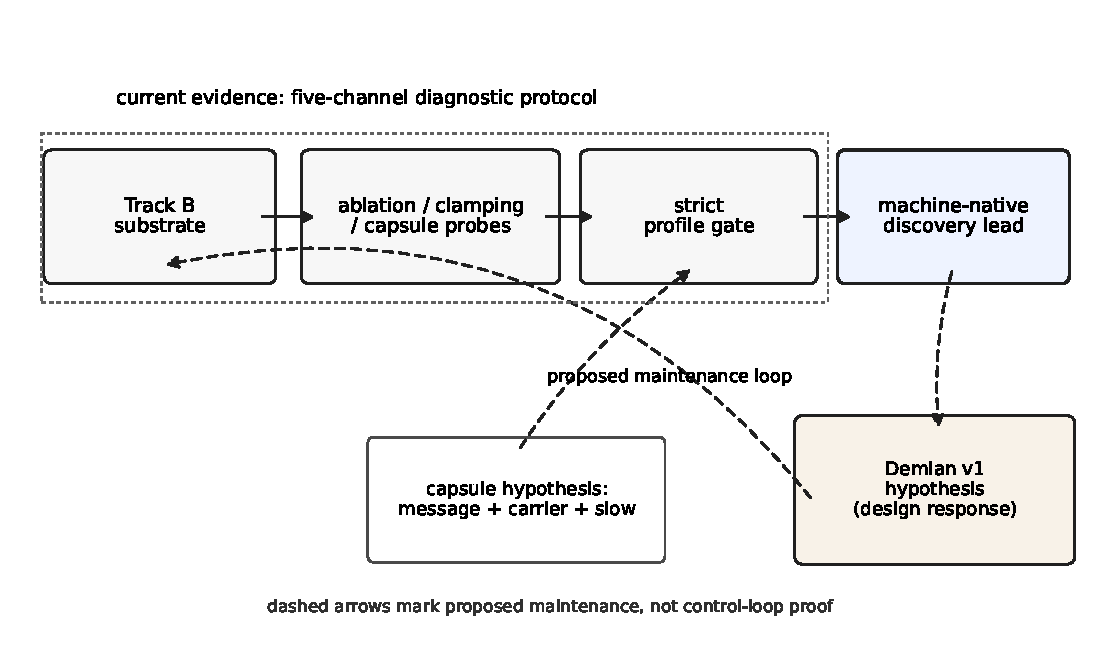
\includegraphics[width=0.84\linewidth]{figures/proposed_maintenance_loop.pdf}
\caption{Operational mechanism schematic and proposed maintenance loop. Solid
arrows summarize the evidence path tested in the current five-channel
diagnostic protocol. The dashed loop is a proposed maintenance loop from the
surviving discovery lead into Demian v1 design hypotheses; it is not presented
as control-loop proof inside the current diagnostic protocol.}
\label{fig:mechanism}
\end{figure}

\section{Diagnostic Protocol}

\subsection{Track B native-emergence search}

The candidates reported here come from Track B native-emergence runs, the
candidate-promotion protocol used for these native-emergence experiments. Track
B is distinct from engineered-target search: instead of selecting only for a
predefined sparse or timed release phenotype, it promotes internally useful
mechanisms that remain supported under causal diagnostics. This distinction is
important because the result reported here is not a sparse-release success.
The replicated top candidates are high-duty phenotypes.

\subsection{Characterization grid}

The focused characterization used seeds 94--102, perturbation scales
0.2, 0.35, and 0.7, two perturbation motifs (\texttt{basis:0} and
\texttt{gaussian:0}), 128 steps, and perturbation step 64. The main focused
artifact is the 2026-05-11 gate-state propagation characterization summary in
the repository's \texttt{data/diagnostics} directory. The replication artifact
is the corresponding 2026-05-11 Track B replication summary.

\subsection{Interventions}

The diagnostic protocol compares the original trajectory against several
interventions:

\begin{description}
  \item[Original] the candidate trajectory without diagnostic ablation.
  \item[Routes-disabled] release-mediated route effects are disabled while the
  rest of the model remains available.
  \item[Gain-zero] explicit release gain is set to zero. The diagnostic also
  checks that gain-zero release-related quantities remain zero within
  tolerance.
  \item[Channel-disabled] a named state channel is zeroed after each step and
  the clamped state is fed into the next step.
\end{description}

The channel-disabled semantics matter. Each step first advances the model;
then the requested channel is zeroed; the row is recorded; the clamped state is
fed forward. This tests whether continuing with that channel removed changes
the trajectory.

\subsection{Mechanism gate}

Gate-State Causal Propagation is the observed case where prior release/gating
history changes later internal evolution, especially through \texttt{message},
\texttt{carrier}, and \texttt{slow} state, even when explicit additive release
gain is zero. The mechanism claim is therefore not that a release vector
directly injects a signal at the diagnostic step; it is that implicit
release/gating state has already shaped the downstream recurrent state so that
ablated continuations diverge from the original.

A candidate passes the mechanism gate when route-disabled and gain-zero
divergence remain positive, gain-zero cleanliness holds, message/carrier
clamping sensitivity repeats, and capsule evidence separates full
internal-state resume from surface-only replay. The gate is intentionally
stricter than reporting surface behavior alone.

\section{Results}

\subsection{Replication summary}

Three Track B native-emergence replications passed the mechanism gate
(Table~\ref{tab:replication}). Held-out route-disabled divergence was positive
in all three runs. Held-out gain-zero divergence was also positive in all three
runs. In this artifact, the mean held-out route-disabled divergence and
mean held-out gain-zero divergence are both 0.2997, with per-run values
0.2422, 0.3194, and 0.3375.

The route-disabled and gain-zero divergence columns are identical in the
current held-out replication summary because, for these selected candidates
and this diagnostic implementation, both interventions expose the same
original-vs-ablated divergence value. The equality is reported rather than
averaged away because it is a useful validity check: gain-zero cleanliness
remains true while the ablated continuation still separates from the original.

\begin{table}[t]
\centering
\caption{Track B Gate-State Causal Propagation replication summary. Values are
from \texttt{gate\_state\_track\_b\_replication\_summary\_20260511}.
Route-disabled and gain-zero are distinct intervention labels in the
diagnostic suite; for these held-out summaries they produced identical
original-vs-ablated divergence values.}
\label{tab:replication}
\begin{tabular}{llllll}
\toprule
Run & Candidate & Duty & Route div. & Gain-zero div. & Gain-zero clean \\
\midrule
1 & \texttt{gen016\_candidate012} & 0.5944 & 0.2422 & 0.2422 & yes \\
2 & \texttt{gen019\_candidate008} & 0.6751 & 0.3194 & 0.3194 & yes \\
3 & \texttt{gen017\_candidate000} & 0.8906 & 0.3375 & 0.3375 & yes \\
\midrule
Mean & -- & -- & 0.2997 & 0.2997 & 3/3 \\
\bottomrule
\end{tabular}
\end{table}

The duty-cycle values reinforce the negative boundary of the result. These are
not low-duty sparse-release candidates; they are high-duty native-emergence
phenotypes that nonetheless preserve a replicated gate-state mechanism under
the current diagnostics.

\subsection{Channel-clamping sensitivity}

The channel-disabled diagnostics identify \texttt{message} and
\texttt{carrier} as the repeated top channels under the clamping intervention
(Table~\ref{tab:channels}).
They were the top two channels in 3/3 replications. The order varied:
\texttt{carrier,message,slow,control} in runs 1 and 3, and
\texttt{message,carrier,control,slow} in run 2. \texttt{slow} support was also
high across the held-out classifications.

\begin{table}[t]
\centering
\caption{Held-out channel-clamping divergences and surface-only resume gaps.}
\label{tab:channels}
\begin{tabular}{lllllll}
\toprule
Run & Message & Carrier & Slow & Control & Order & Surface gap \\
\midrule
1 & 1.1289 & 1.2604 & 0.8589 & 0.6411 &
\texttt{carrier,message,slow,control} & 0.6637 \\
2 & 1.0852 & 0.8930 & 0.8101 & 0.8720 &
\texttt{message,carrier,control,slow} & 0.7789 \\
3 & 1.0187 & 1.1618 & 0.8553 & 0.6475 &
\texttt{carrier,message,slow,control} & 0.3565 \\
\bottomrule
\end{tabular}
\end{table}

The repeated message/carrier pattern is the strongest channel-level evidence
for the mechanism under this intervention. Because clamping a channel to zero
is a strong out-of-distribution intervention, we read these values as
channel-clamping sensitivity under the reported protocol, not as a general
proof that no other representation could carry the same function. The pattern
still suggests that the effect is not localized only in the readout-adjacent
\texttt{fast} surface, nor explained solely by the persistent \texttt{slow}
accumulator.

\subsection{Gain-zero and route-disabled behavior}

The gain-zero diagnostic is designed to distinguish a simple additive release
effect from a more stateful gate-history effect. In the focused
characterization, gain-zero cleanliness is true: release strength, route norm,
and endogenous release norm are zero under the gain-zero condition within the
recorded tolerance. Yet original-vs-gain-zero divergence remains positive and
matches the route-disabled divergence in the held-out replication rows.

This pattern motivates the name Gate-State Causal Propagation. The observed
effect is not that a nonzero release vector directly injects a signal under
gain-zero. Rather, the candidate's release/gating history embedded in recurrent
state appears to alter
later dynamics in a way that remains visible under the diagnostic comparison.
The result should therefore be separated from a route-specific sparse-release
claim.

\subsection{Reduced matched control comparison}

We added a matched control/null comparison using the same route-disabled,
gain-zero, channel-clamping, and capsule criteria. The reduced grid used seeds
96--98, perturbation scale 0.35, motifs \texttt{basis:0} and
\texttt{gaussian:0}, and the same seven intervention conditions. The binary
gate was not selective by itself: the default unselected control passed in
1/1 case and random unselected controls passed in 15/32 cases. We therefore
report a stricter Track-B-calibrated descriptive profile, using the weakest
Track B positive as the threshold. This profile is not a pre-registered
discovery criterion; it is a post hoc effect-size summary used to test whether
the replicated positives occupy a more selective region than random unselected
controls. It requires the binary gate, route/gain-zero divergence at least as
large as the weakest Track B positive, and message/carrier clamping dominance
over slow/control at least as large as the weakest Track B positive. Under that
stricter profile, Track B positives passed in 3/3 cases, the default unselected
control passed in 0/1, and random unselected controls passed in 2/32
(Table~\ref{tab:controls}). The Track B versus random enrichment factor was
16.0, with one-sided Fisher exact \(p=0.00153\).

\begin{table}[t]
\centering
\caption{Reduced matched control/null comparison from
\texttt{gate\_state\_control\_nulls\_20260515}. The binary gate is broad; the
strict descriptive profile adds Track-B-calibrated effect-size and channel-dominance
criteria.}
\label{tab:controls}
\begin{tabular}{llllll}
\toprule
Family & N & Binary pass & Strict pass & Route div. & M/C dom. \\
\midrule
Track B positives & 3 & 3/3 & 3/3 & 0.2994 & 0.3104 \\
Default unselected & 1 & 1/1 & 0/1 & 0.1528 & 0.3597 \\
Random unselected & 32 & 15/32 & 2/32 & 0.1398 & 0.2033 \\
\bottomrule
\end{tabular}
\end{table}

This control result changes the interpretation. The Track B candidates remain
replicated positives under the diagnostic protocol, but the original binary
gate cannot support a rarity or discovery-specificity claim. The stricter
descriptive profile gives a stronger artifact: it sharply reduces
random-control passes while preserving all three Track B positives. Because the
profile is post hoc, its remaining false positives show that larger null
populations, pre-specified thresholds, and independent replications are still
required before treating the profile as rare.

\subsection{Capsule continuity}

Surface-only replay was insufficient to resume the trajectory. Full
internal-state resume was exact in 3/3 replications, as expected for a
deterministic full-state continuation, while surface-only resume left a
positive final gap in 3/3. The surface-only gaps were 0.6637, 0.7789, and
0.3565. The focused characterization also reports exact full-internal-state
resume over 54 capsule runs for the representative candidate: full internal
state and uninterrupted continuation both have zero final L2 gap and zero
mean-step gap, while surface-only replay has positive final and mean-step
gaps.

This result should be read narrowly. It shows that, under this deterministic
probe, the complete internal state resumes the trajectory while surface-only
replay does not. It does not show that the state has been compressed, nor that
the capsule is minimal.

\section{Discussion}

The result supports an internal-state-centered view of this substrate. The
release/gating subsystem is not only an output-side switch; its history can be
part of the downstream computation. The repeated sensitivity of
\texttt{message} and \texttt{carrier} under channel clamping further suggests
that the mechanism depends on routed intermediate state rather than on the
readout surface alone.

The capsule-continuity result gives a complementary test of surface
insufficiency. Full-state resume is expected to be exact in a deterministic
RNN-style system, so the informative comparison is the failure of surface-only
replay. If surface state were sufficient for this computation under the probe,
surface-only replay should resume the trajectory as well as full internal-state
continuation. It does not. The stronger conclusion is not that full-state
copying is a useful compression method, but that evaluation based only on the
exposed readout would miss the state needed for continuation.

This result also motivates an architectural response: make gate state explicit
in Demian v1. The current Demian v1 prototype exists as a six-channel
architecture with \texttt{fast}, \texttt{slow}, \texttt{control},
\texttt{message}, \texttt{carrier}, and \texttt{gate} state. Its gate channel
modulates message-carrier, carrier-slow, and message/carrier-surface routes
without injecting an additive release vector. That prototype is a design
response with unit-level architectural tests, not a validated empirical result
of this paper. The present evidence supports a narrower claim: in the current
v9 five-channel Track B protocol, gate-state propagation replicated and
survived the reported ablation and resume tests.

This is the sense in which we treat the result as a discovery lead rather than
a closed discovery claim. The lead was not supplied by a human benchmark target
or by an externally imposed human-facing objective. It emerged from a
machine-native state trajectory, survived a first replication and ablation
round, weakened under broad controls, and then sharpened into an enriched
message/carrier-dominant profile. Demian v1 is therefore framed as a
design response to the substrate's own diagnostic signal, not as proof that the
signal has already been fully explained.

As a lab interpretation, Demian is best understood here as an experimental
substrate workflow, not just a model instance. The workflow discovers native
signals in a structured recurrent substrate, applies ablations and controls to
separate robust internal-state structure from surface coincidence, and then
turns the surviving profile into the next design hypothesis. In the lab
timeline, related probes moved from transformer-style state inspection through
Mamba-like sequence-state experiments and then into explicit recurrent
substrates such as vanilla RNN, GRU, and LSTM-style scaffolds; the present
five-channel substrate is the point where the message/carrier/slow capsule
hypothesis became experimentally inspectable. In this paper, that means a
replicated machine-native discovery lead, enriched under the strict
Track-B-profile gate, motivates Demian v1 without validating it.

\section{Limitations}

The result is limited to the current substrate family and current Track B
protocol. It has not yet been shown to be universal across recurrent
architectures, independent implementations, or broader search spaces. The
replicated candidates are high-duty phenotypes, so this paper does not validate
the original sparse delayed-release target.

The current evidence is also selected-candidate evidence. The reduced matched
control comparison shows that the binary mechanism gate has high background
pass rates in unselected controls, while the stricter profile gate reduces but
does not eliminate random-control passes. The capsule evidence is full-state
evidence: it shows surface insufficiency under this probe, not a minimal or
compressed memory. Broader tests should use larger matched control
populations, stronger held-out sets, and independent reimplementations of the
diagnostic protocol.

\section{Reproducibility}

The public repository is:

\begin{quote}
\url{https://github.com/Aeshma-Daeva/Demian}
\end{quote}

The compact local test path for the core Gate-State result is:

\begin{verbatim}
./venv/bin/python -m pytest \
  tests/test_gate_state_propagation_characterization.py \
  tests/test_v9_capsule_continuity.py \
  tests/test_gate_state_control_nulls.py -q
\end{verbatim}

The main replication artifact can be inspected with:

\begin{verbatim}
./venv/bin/python - <<'PY'
import json
from pathlib import Path

summary = json.loads(Path(
    "data/diagnostics/gate_state_track_b_replication_summary_20260511/"
    "summary.json"
).read_text())
print(json.dumps({
    "replication_count": summary.get("replication_count"),
    "passed_replication_count": summary.get("passed_replication_count"),
    "message_carrier_top2_count": summary.get("message_carrier_top2_count"),
    "mean_heldout_routes_divergence": summary.get(
        "mean_heldout_routes_divergence"
    ),
    "mean_heldout_gain_zero_divergence": summary.get(
        "mean_heldout_gain_zero_divergence"
    ),
}, indent=2, sort_keys=True))
PY
\end{verbatim}

Primary artifacts under \texttt{data/diagnostics}:

\begin{itemize}
  \item \texttt{gate\_state\_propagation\_characterization\_20260511/summary.json}
  \item \texttt{gate\_state\_track\_b\_replication\_summary\_20260511/summary.json}
  \item \texttt{gate\_state\_track\_b\_replication\_1\_heldout\_20260511/summary.json}
  \item \texttt{gate\_state\_track\_b\_replication\_2\_heldout\_20260511/summary.json}
  \item \texttt{gate\_state\_track\_b\_replication\_3\_heldout\_20260511/summary.json}
  \item \texttt{gate\_state\_control\_nulls\_20260515/control\_null\_summary.json}
  \item \texttt{../substrate\_lab/v9\_capsule\_continuity\_20260511/summary.json}
\end{itemize}

Exact paths are listed in the repository artifact index and manifest.

\section{Conclusion}

Gate-State Causal Propagation is a replicated internal mechanism in the current
structured recurrent substrate protocol. Across three Track B replications,
the mechanism preserved positive held-out route-disabled and gain-zero
divergence, clean gain-zero diagnostics, repeated message/carrier
channel-clamping sensitivity, and exact full internal-state resume with
positive surface-only resume gaps.

The result is intentionally bounded. It is not a sparse-release success claim,
not a benchmark-superiority claim, not a final rarity claim, and not a
validation of a final architecture. Its value is narrower and more concrete:
it identifies a replicated internal-state diagnostic pattern, shows that a
strict Track-B-calibrated descriptive profile is enriched over random
unselected controls, and turns a replicated machine-native discovery lead into
a testable architectural motivation for Demian v1 and later gate-state
experiments.

\bibliographystyle{plainnat}
\bibliography{references}

\end{document}
